\documentclass{scrartcl}
        \usepackage{xcolor, tikz}
        \usepackage{pgfplots}
        \pgfplotsset{compat=newest}
        \pagestyle{empty}
        \definecolor{pdg2112}{RGB}{228,26,28}
\definecolor{pdg2212}{RGB}{55,126,184}
\definecolor{pdg1000010020}{RGB}{153,153,153}
\definecolor{pdg1000020040}{RGB}{166,86,40}
\definecolor{pdg11}{RGB}{152,78,163}
\definecolor{pdg22}{RGB}{77,175,74}
\definecolor{pdg1000060120}{RGB}{153,153,153}
\definecolor{pdg1000040090}{RGB}{153,153,153}
\begin{document}
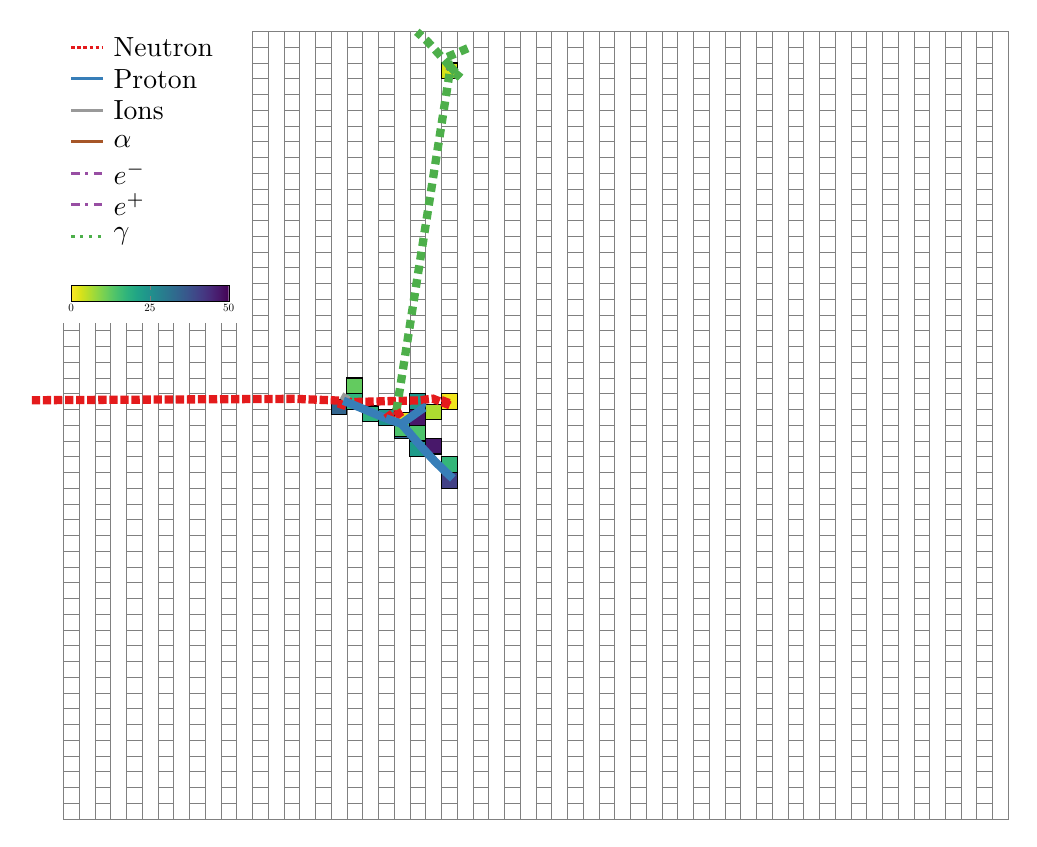
\begin{tikzpicture}[scale=0.4] %\columnwidth/252.0pt]
\draw[step=0.5,very thin,gray] (-0.001000,-12.499) grid (0.500000,3.25);
\draw[step=0.5,very thin,gray] (0.999000,-12.499) grid (1.500000,3.25);
\draw[step=0.5,very thin,gray] (1.999000,-12.499) grid (2.500000,3.25);
\draw[step=0.5,very thin,gray] (2.999000,-12.499) grid (3.500000,3.25);
\draw[step=0.5,very thin,gray] (3.999000,-12.499) grid (4.500000,3.25);
\draw[step=0.5,very thin,gray] (4.999000,-12.499) grid (5.500000,3.25);
\draw[step=0.5,very thin,gray] (5.999000,-12.499) grid (6.500000,12.499);
\draw[step=0.5,very thin,gray] (6.999000,-12.499) grid (7.500000,12.499);
\draw[step=0.5,very thin,gray] (7.999000,-12.499) grid (8.500000,12.499);
\draw[step=0.5,very thin,gray] (8.999000,-12.499) grid (9.500000,12.499);
\draw[step=0.5,very thin,gray] (9.999000,-12.499) grid (10.500000,12.499);
\draw[step=0.5,very thin,gray] (10.999000,-12.499) grid (11.500000,12.499);
\draw[step=0.5,very thin,gray] (11.999000,-12.499) grid (12.500000,12.499);
\draw[step=0.5,very thin,gray] (12.999000,-12.499) grid (13.500000,12.499);
\draw[step=0.5,very thin,gray] (13.999000,-12.499) grid (14.500000,12.499);
\draw[step=0.5,very thin,gray] (14.999000,-12.499) grid (15.500000,12.499);
\draw[step=0.5,very thin,gray] (15.999000,-12.499) grid (16.500000,12.499);
\draw[step=0.5,very thin,gray] (16.999000,-12.499) grid (17.500000,12.499);
\draw[step=0.5,very thin,gray] (17.999000,-12.499) grid (18.500000,12.499);
\draw[step=0.5,very thin,gray] (18.999000,-12.499) grid (19.500000,12.499);
\draw[step=0.5,very thin,gray] (19.999000,-12.499) grid (20.500000,12.499);
\draw[step=0.5,very thin,gray] (20.999000,-12.499) grid (21.500000,12.499);
\draw[step=0.5,very thin,gray] (21.999000,-12.499) grid (22.500000,12.499);
\draw[step=0.5,very thin,gray] (22.999000,-12.499) grid (23.500000,12.499);
\draw[step=0.5,very thin,gray] (23.999000,-12.499) grid (24.500000,12.499);
\draw[step=0.5,very thin,gray] (24.999000,-12.499) grid (25.500000,12.499);
\draw[step=0.5,very thin,gray] (25.999000,-12.499) grid (26.500000,12.499);
\draw[step=0.5,very thin,gray] (26.999000,-12.499) grid (27.500000,12.499);
\draw[step=0.5,very thin,gray] (27.999000,-12.499) grid (28.500000,12.499);
\draw[step=0.5,very thin,gray] (28.999000,-12.499) grid (29.500000,12.499);
\draw[very thin,gray] (0,-12.5) -- (30,-12.5) -- (30,12.5) -- (6,12.5);
\definecolor{tempcolor}{rgb}{0.195860,0.395433,0.555276}\draw[fill=tempcolor,fill opacity=1] (8.500000,0.326999) rectangle (9.000000,0.826999);
\definecolor{tempcolor}{rgb}{0.191090,0.708366,0.482284}\draw[fill=tempcolor,fill opacity=1] (9.000000,0.500000) rectangle (9.500000,1.000000);
\definecolor{tempcolor}{rgb}{0.386433,0.794644,0.372886}\draw[fill=tempcolor,fill opacity=1] (9.000000,1.000000) rectangle (9.500000,1.500000);
\definecolor{tempcolor}{rgb}{0.175707,0.697900,0.491033}\draw[fill=tempcolor,fill opacity=1] (9.500000,0.109818) rectangle (10.000000,0.609818);
\definecolor{tempcolor}{rgb}{0.122606,0.585371,0.546557}\draw[fill=tempcolor,fill opacity=1] (10.000000,0.000000) rectangle (10.500000,0.500000);
\definecolor{tempcolor}{rgb}{0.926106,0.897330,0.104071}\draw[fill=tempcolor,fill opacity=1] (10.500000,-0.088422) rectangle (11.000000,0.411578);
\definecolor{tempcolor}{rgb}{0.201239,0.383670,0.554294}\draw[fill=tempcolor,fill opacity=1] (10.500000,-0.432059) rectangle (11.000000,0.067941);
\definecolor{tempcolor}{rgb}{0.296479,0.761561,0.424223}\draw[fill=tempcolor,fill opacity=1] (10.500000,-0.347299) rectangle (11.000000,0.152701);
\definecolor{tempcolor}{rgb}{0.119512,0.607464,0.540218}\draw[fill=tempcolor,fill opacity=1] (11.000000,-1.000000) rectangle (11.500000,-0.500000);
\definecolor{tempcolor}{rgb}{0.296479,0.761561,0.424223}\draw[fill=tempcolor,fill opacity=1] (11.000000,-0.500000) rectangle (11.500000,0.000000);
\definecolor{tempcolor}{rgb}{0.281924,0.089666,0.412415}\draw[fill=tempcolor,fill opacity=1] (11.000000,0.000000) rectangle (11.500000,0.500000);
\definecolor{tempcolor}{rgb}{0.121148,0.592739,0.544641}\draw[fill=tempcolor,fill opacity=1] (11.000000,0.500000) rectangle (11.500000,1.000000);
\definecolor{tempcolor}{rgb}{0.282327,0.094955,0.417331}\draw[fill=tempcolor,fill opacity=1] (11.500000,-0.914212) rectangle (12.000000,-0.414212);
\definecolor{tempcolor}{rgb}{0.678489,0.863742,0.189503}\draw[fill=tempcolor,fill opacity=1] (11.500000,0.168595) rectangle (12.000000,0.668595);
\definecolor{tempcolor}{rgb}{0.257322,0.256130,0.526563}\draw[fill=tempcolor,fill opacity=1] (12.000000,-2.000000) rectangle (12.500000,-1.500000);
\definecolor{tempcolor}{rgb}{0.202219,0.715272,0.476084}\draw[fill=tempcolor,fill opacity=1] (12.000000,-1.500000) rectangle (12.500000,-1.000000);
\definecolor{tempcolor}{rgb}{0.945636,0.899815,0.112838}\draw[fill=tempcolor,fill opacity=1] (12.000000,0.500000) rectangle (12.500000,1.000000);
\definecolor{tempcolor}{rgb}{0.835270,0.886029,0.102646}\draw[fill=tempcolor,fill opacity=1] (12.000000,11.000000) rectangle (12.500000,11.500000);
\draw[color=pdg2112, line width=3pt, densely dotted] (-1.002145195933099, 0.7929280659188469) -- (-0.002159593221222167, 0.7982497307907855) -- (0.48999999999998634, 0.80086887691802) -- (0.9899999999999863, 0.8035297476633119) -- (1.4899999999999864, 0.806190618408604) -- (1.9899999999999864, 0.8088514891538958) -- (2.4899999999999864, 0.8115123598991877) -- (2.9899999999999864, 0.8141732306444798) -- (3.4899999999999864, 0.8168341013897716) -- (3.9899999999999864, 0.8194949721350637) -- (4.489999999999986, 0.8221558428803556) -- (4.989999999999986, 0.8248167136256475) -- (5.489999999999986, 0.8274775843709395) -- (5.989999999999986, 0.8301384551162314) -- (6.489999999999986, 0.8327993258615235) -- (6.989999999999986, 0.8354601966068154) -- (7.347364524855766, 0.8373619982260033) -- (7.490000000000009, 0.8317277572476491) -- (7.990000000000009, 0.8119772675021751) -- (8.490000000000009, 0.7922267777567011) -- (8.889300298023045, 0.7764540248737631);
\draw[color=pdg1000020040, line width=3pt, solid] (8.889300298023045, 0.7764540248737631);
\draw[color=pdg2112, line width=3pt, densely dotted] (8.889300298023045, 0.7764540248737631) -- (8.792455403978966, 0.4863019276237536);
\draw[color=pdg2212, line width=3pt, solid] (8.792455403978966, 0.4863019276237536);
\draw[color=pdg1000020040, line width=3pt, solid] (8.889300298023045, 0.7764540248737631);
\draw[color=pdg2112, line width=3pt, densely dotted] (8.889300298023045, 0.7764540248737631) -- (8.990000000000009, 0.7601750691792717) -- (9.146457793380796, 0.7348823479844612) -- (9.489999999999986, 0.7433276597883394) -- (9.51411562293481, 0.7439204951113514) -- (9.522820988603645, 0.7441344994637233) -- (9.990000000000009, 0.7556191797837847) -- (10.490000000000009, 0.7679106997792292) -- (10.990000000000009, 0.7802022197746737) -- (11.354322033596258, 0.7891583628961327) -- (11.470946674761603, 0.811474114941135) -- (11.490000000000009, 0.8136614240228981) -- (11.734305428304447, 0.8417075249196293) -- (11.989999999999986, 0.7410236641240987) -- (12.277007583088857, 0.6280098001560059) -- (12.214959941742109, 0.6226520051767437) -- (12.13147293441998, 0.7771410454042839) -- (12.168541545763242, 0.8772370866853582);
\draw[color=pdg2212, line width=3pt, solid] (12.168541545763242, 0.8772370866853582);
\draw[color=pdg2212, line width=3pt, solid] (12.13147293441998, 0.7771410454042839);
\draw[color=pdg1000060120, line width=3pt, solid] (12.277007583088857, 0.6280098001560059);
\draw[color=pdg2212, line width=3pt, solid] (11.354322033596258, 0.7891583628961327);
\draw[color=pdg1000060120, line width=3pt, solid] (9.146457793380796, 0.7348823479844612);
\draw[color=pdg1000010020, line width=3pt, solid] (8.889300298023045, 0.7764540248737631) -- (8.92006375517094, 0.8290777290035146) -- (8.944362559102752, 0.8717380644057615) -- (8.963935371467505, 0.9058737247326386) -- (8.979790363896587, 0.933102783011831) -- (8.989999999999986, 0.9503170085166145) -- (9.002999999999997, 0.972527499708225);
\draw[color=pdg2212, line width=3pt, solid] (8.889300298023045, 0.7764540248737631) -- (8.990000000000009, 0.735484728460868) -- (9.490000000000009, 0.5299984560913209) -- (9.989999999999986, 0.32127360102968483) -- (10.239218763180087, 0.21654468612676445);
\draw[color=pdg1000040090, line width=3pt, solid] (10.239218763180087, 0.21654468612676445);
\draw[color=pdg2212, line width=3pt, solid] (10.239218763180087, 0.21654468612676445);
\draw[color=pdg2212, line width=3pt, solid] (10.239218763180087, 0.21654468612676445);
\draw[color=pdg2112, line width=3pt, densely dotted] (10.239218763180087, 0.21654468612676445) -- (10.490000000000009, 0.40642208883248665) -- (10.497000000000025, 0.4117220938719215) -- (10.502999999999997, 0.4162649553342795) -- (10.508000000000015, 0.4200506732195974) -- (10.577104979849878, 0.4723730648558752);
\draw[color=pdg22, line width=3pt, dotted] (10.577104979849878, 0.4723730648558752) -- (10.877155650775808, 2.379341185538851) -- (10.881865315216487, 2.4092733963876287) -- (10.885902170451345, 2.4349295771151533) -- (10.889266216480404, 2.4563097277214236) -- (10.989999999999986, 3.0965219733892324) -- (10.992000000000008, 3.109232947271095) -- (10.99699999999998, 3.141010381975572) -- (11.002999999999975, 3.1791433036211396) -- (11.007999999999992, 3.210920738325825) -- (11.010000000000014, 3.223631712207647) -- (11.051911546710539, 3.4899999999999998) -- (11.13058372472742, 3.9900000000000007) -- (11.209255902744326, 4.49) -- (11.28792808076123, 4.99) -- (11.366600258778112, 5.49) -- (11.445272436795017, 5.99) -- (11.489999999999986, 6.274265443848407) -- (11.492000000000008, 6.286976417730268) -- (11.49699999999998, 6.318753852434745) -- (11.502999999999975, 6.356886774080313) -- (11.507999999999992, 6.388664208784999) -- (11.510000000000014, 6.401375182666821) -- (11.549964856585712, 6.6553713067928655) -- (11.55467452102639, 6.685303517641644) -- (11.558711376261249, 6.710959698369169) -- (11.56207542229031, 6.73233984897544) -- (11.886369459490743, 8.793386367419874) -- (11.891079123931423, 8.823318578268651) -- (11.895115979166281, 8.848974758996174) -- (11.89848002519534, 8.870354909602446) -- (11.989999999999986, 9.452008914306385) -- (11.992000000000008, 9.464719888188245) -- (11.99699999999998, 9.496497322892724) -- (12.002999999999975, 9.53463024453829) -- (12.007999999999992, 9.566407679242976) -- (12.010000000000014, 9.579118653124798) -- (12.074649860930412, 9.989999999999998) -- (12.153322038947318, 10.49) -- (12.2319942169642, 10.99) -- (12.273178578986949, 11.251746675005664);
\draw[color=pdg11, line width=3pt, dashdotted] (12.273178578986949, 11.251746675005664) -- (12.28214050337574, 11.297256738135072) -- (12.279985262770287, 11.333473818840428) -- (12.272760458600237, 11.359913007099777) -- (12.270135746258166, 11.382504134784853) -- (12.274960500327234, 11.39467945389125);
\draw[color=pdg22, line width=3pt, dotted] (12.274666841481736, 11.399672063850591) -- (12.489999999999986, 11.163409965007382) -- (12.60372605485379, 11.038630499560421) -- (12.509999999999991, 11.115315732113453) -- (12.321868919757389, 11.269241720584432) -- (12.234684102168035, 11.49) -- (12.166277432276434, 11.663210647947329) -- (12.176387881529877, 11.68541736838808) -- (12.489999999999986, 11.819323478827284) -- (12.656017550093157, 11.890209656651246) -- (12.666611098519137, 11.89473289023161) -- (12.693094969584104, 11.906040974182519) -- (12.724875614862048, 11.919610674923607) -- (12.751359485927015, 11.930918758874515) -- (12.761953034352995, 11.935441992454876) -- (12.96748226882671, 12.0231988702955);
\draw[color=pdg11, line width=3pt, dashdotted] (12.60372605485379, 11.038630499560421);
\draw[color=pdg22, line width=3pt, dotted] (12.274666841481736, 11.399672063850591) -- (12.192340476445953, 11.49) -- (12.009999999999991, 11.69006274911688) -- (11.558418615314167, 12.185534818901896) -- (11.510000000000014, 12.22947680001849) -- (11.22293573298732, 12.489999999999998);
\draw[color=pdg1000060120, line width=3pt, solid] (10.577104979849878, 0.4723730648558752);
\draw[color=pdg2112, line width=3pt, densely dotted] (10.577104979849878, 0.4723730648558752) -- (10.708364444831137, 0.25257138969321347) -- (10.727120297856164, 0.2278662742344712) -- (10.670978700524506, 0.286569785400388);
\draw[color=pdg2212, line width=3pt, solid] (10.670978700524506, 0.286569785400388);
\draw[color=pdg2212, line width=3pt, solid] (10.708364444831137, 0.25257138969321347);
\draw[color=pdg2212, line width=3pt, solid] (10.239218763180087, 0.21654468612676445) -- (10.490000000000009, 0.1292207755481459) -- (10.733803756095085, 0.04424821754494281) -- (10.836173207829802, 0.1210880630081925) -- (10.982674602655766, 0.22658495591370492) -- (10.989999999999986, 0.2317766598077849) -- (11.002999999999997, 0.24100116966852508) -- (11.109335394858771, 0.3155185410845242) -- (11.1895115512071, 0.3726988200318047) -- (11.254101862143376, 0.4189942620936768) -- (11.304792124852678, 0.4548610728849158) -- (11.34516407574456, 0.4833414154185485) -- (11.355178149915492, 0.48999999999999994) -- (11.365934423669364, 0.497) -- (11.37521584473393, 0.5030000000000001) -- (11.382950362287739, 0.5079999999999999) -- (11.411306661650361, 0.5257494092749082) -- (11.431555889113042, 0.538499071829672) -- (11.447939312876134, 0.5489701363567454) -- (11.461073533675062, 0.5573648758915095) -- (11.478007641150134, 0.5557414579073638) -- (11.48803822170414, 0.552385593216334);
\draw[color=pdg2212, line width=3pt, solid] (10.733803756095085, 0.04424821754494281) -- (10.989999999999986, -0.2513621452539323) -- (11.196213806063952, -0.49000000000000005) -- (11.439474664169392, -0.7653174689202247) -- (11.490000000000009, -0.821070336293853) -- (11.680885289692174, -1.026434504172051) -- (11.817518422066678, -1.1699873559502099) -- (11.931081297190554, -1.2805207658241173) -- (11.989999999999986, -1.3389992630189043) -- (12.085935621503314, -1.4334335650286179) -- (12.145454964987675, -1.49) -- (12.212651368425714, -1.5522978693334253) -- (12.249916525614253, -1.5860406448934865) -- (12.278994730288128, -1.613641740880794) -- (12.302625591788182, -1.6352830865011765) -- (12.321247403259463, -1.652455777908612) -- (12.33592836408227, -1.6664130969206865) -- (12.347601084233428, -1.67757066624505) -- (12.356933519180256, -1.6861350558762804) -- (12.364403028677362, -1.6930850361861327);
\draw[color=pdg2112, very thick, densely dotted] (0.25,12) -- (1.25,12) node [right,black] {Neutron};
\draw[color=pdg2212, very thick, solid] (0.25,11) -- (1.25,11) node [right,black] {Proton};
\draw[color=pdg1000010020, very thick, solid] (0.25,10) -- (1.25,10) node [right,black] {Ions};
\draw[color=pdg1000020040, very thick, solid] (0.25,9) -- (1.25,9) node [right,black] {$\alpha$};
\draw[color=pdg11, very thick, dashdotted] (0.25,8) -- (1.25,8) node [right,black] {$e^-$};
\draw[color=pdg11, very thick, dashdotted] (0.25,7) -- (1.25,7) node [right,black] {$e^+$};
\draw[color=pdg22, very thick, dotted] (0.25,6) -- (1.25,6) node [right,black] {$\gamma$};

        \begin{axis}[%
            at={(0.25cm,4.75cm)},
            hide axis,
            scale only axis,
            height=0pt,
            width=0pt,
            colormap={reverse viridis}{
                indices of colormap={
                \pgfplotscolormaplastindexof{viridis},...,0 of viridis}
            },
            colorbar horizontal,
            point meta min=0,
            point meta max=50,
            colorbar style={
                width=5cm,
                xtick={50, 25, 0},
            }]
        \end{axis}
        
        \end{tikzpicture}
        \end{document}
        